\documentclass{beamer}
\usepackage[fontset=adobe]{ctex}
\usetheme{Boadilla}
\setbeamercovered{dynamic}
\title{基于公众关注度的股票市场的分析与预测}
\subtitle{综合论文训练答辩}
\author{李雨田}
\institute{清华大学}
\begin{document}

\begin{frame}
\titlepage
\begin{center}
  \begin{tabular}{ll}
    指导老师 & 余宏亮 \\
    报告人 & 李雨田 \\
    学号 & 2010012193
  \end{tabular}
\end{center}
\end{frame}

\begin{frame}{数据获取及预处理}{目的}
\begin{itemize}
  \item 统一数据结构
  \pause
  \item 高效率
  \pause
  \item 易用
\end{itemize}
\end{frame}

\begin{frame}{数据获取及预处理}{框架}
\begin{itemize}
  \item 基于 JSON 和 Redis 数据库
  \pause
  \item 基于事件循环机制
  \pause
  \item 提供 JavaScript 和 Python 库,与 Numpy , Pandas 和 StatsModels 对接
\end{itemize}
\end{frame}

\begin{frame}{数据来源}
\begin{itemize}
  \item 挑选上证 50 指数成分股
  \pause
  \item 从东方财富网股吧获取用户关注度数据
  \begin{itemize}
    \item 个股所有讨论帖点击量
    \item 对应的时间和内容
  \end{itemize}
  \pause
  \item 从国信证券客户端获取历史股票价格和交易量
\end{itemize}
\end{frame}

\begin{frame}{情感分析}
\begin{itemize}
  \item 拼接讨论帖标题和内容,去除非中文字符,使用翻译 API 翻译成英文
  \pause
  \item 使用卷积神经网络分析情感,该模型基于 Twitter 数据训练得到
\end{itemize}
\end{frame}

\begin{frame}{情感分析}
\begin{figure}
  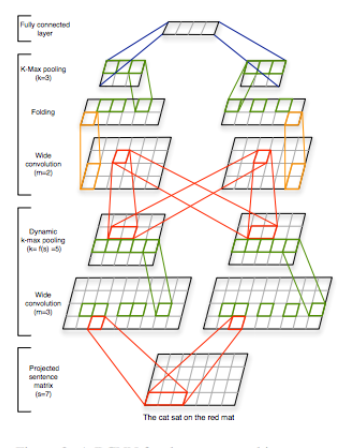
\includegraphics[width=0.4\textwidth]{0.png}
  \caption{情感分析卷积神经网络}
\end{figure}
\end{frame}

\begin{frame}{因果关系分析}{格兰杰因果关系}
\begin{block}{假设检验}
  \[
    y_{t}=a_{0}+\sum_{i=1}^{m}a_{i}y_{t-i}+\sum_{i=1}^{m}b_{i}x_{t-i}+residual_{t}
  \]
  \[
    H_{0}:b_{1}=b_{2}=\cdots =b_{m}=0
  \]
\end{block}
\end{frame}

\begin{frame}{预测模型}
\end{frame}

\end{document}